\documentclass[conference]{IEEEtran}
\usepackage{graphicx}
\usepackage{amsmath}
\usepackage{url}
\begin{document}

\title{Redstone Cortex: An Atlas-Mapped Winner-Take-All Circuit with a Physical Redstone Neuron in Vanilla Minecraft}
\author{\IEEEauthorblockN{Devansh Gaur}
\IEEEauthorblockA{University of Waterloo, Waterloo, ON, Canada}}
\maketitle

\begin{figure*}[t]
\centering
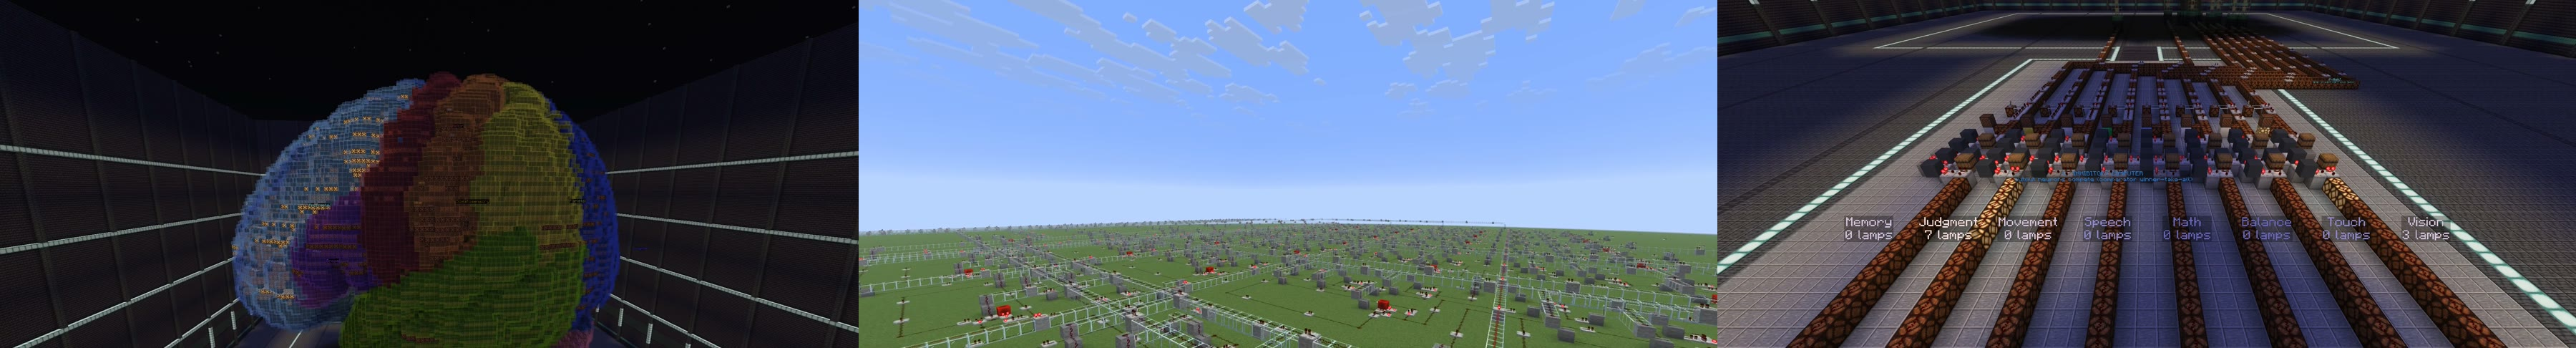
\includegraphics[width=\textwidth]{fig1.jpg}
\caption{Frames from one recorded run, left to right (a) to (c), of the question ``who would win in a fight jensen huang or elon musk?''. (a) The 519,814-voxel brain with the prefrontal region lit. (b) The physical redstone neuron (49,164 blocks) during its 144 s evaluation, while the brain's clock is paused. (c) The comparator winner-take-all board. Floating tags give the number of lit lamps on each region's bar, read from the lamp blocks; the judgment (prefrontal) bar holds 7 lamps after the other bars are cut.}
\label{fig:frames}
\end{figure*}

\begin{abstract}
Minecraft redstone is a set of discrete signal components with integer strengths from 0 to 15. We used it to build a didactic model of cortical routing in the unmodified game. A question typed on an in-game sign is converted to eight category inputs, passed through a 16-unit integer network of leaky integrators with global inhibition, and resolved by a winner-take-all circuit made of redstone comparators. The winning signal travels along a redstone axon and lights the matching region of a 120 x 106 x 96-block brain built from the MNI152 template and the Harvard-Oxford atlas. One hidden unit, the prefrontal (judgment) detector, is computed by a physical redstone neuron of 49,164 blocks built on a carry-save multiply-accumulate unit; the game's command system only writes its inputs and reads its output lamps. The neuron matched a tick-level simulator on 10 of 10 test cases and was correct on 24 of 24 cases from 20 to 100 game ticks per second. One evaluation takes 144 s at the default rate, and about 151 s inside the brain. The comparator winner-take-all selected the correct region on 25 of 25 test vectors, including ties.
\end{abstract}

\begin{IEEEkeywords}
Minecraft, redstone, winner-take-all, neuromorphic hardware, brain atlas, education.
\end{IEEEkeywords}

\section{Introduction}
Popular accounts of the brain often say that a given kind of thought ``happens'' in a given region. This project turns that claim into a visible machine and states where the analogy fails. The target was a model a viewer can watch end to end: a question goes in, discrete signals compete, and one region lights. Redstone suits this because its signals are integers from 0 to 15 that decay by one per block of wire, and its comparators subtract or compare two such signals. These are the operations a small integer network needs. The project also asked how much of the computation can be moved out of the game's command system and into redstone itself.

\section{Related Work}
Threshold units date to McCulloch and Pitts~\cite{mp}, and winner-take-all selection is a standard model of competition through lateral inhibition with known computational power~\cite{maass}. Neuromorphic engineering builds such units in physical hardware rather than software~\cite{mead}. Minecraft has served as an artificial intelligence research platform~\cite{malmo}, where the game is an environment for an external agent. Here the game itself is the computing substrate. Our multiplier uses carry-save accumulation~\cite{wallace} to remove the carry chain, the slowest path in redstone. The brain geometry uses the MNI152 template~\cite{fonov} and Harvard-Oxford labels~\cite{desikan}, loaded with nilearn~\cite{nilearn}.

\section{System}
\subsection{Anatomy}
Grey and white matter templates were thresholded and sampled at 1.5 mm per block, giving 519,814 voxels with sulci carved by cerebrospinal fluid. Harvard-Oxford labels were grouped into eight regions: prefrontal, Broca, motor, somatosensory, parietal, temporal, occipital and cerebellum (derived from unlabelled inferior voxels). The outer shell is region-coloured glass. Each region of the left hemisphere is lit by a torch ladder that powers horizontal plates of redstone dust on lamps every four levels; lamps beside a powered plate light the visible surface. On the prefrontal region, dust on every plate row lights 25.9\% of its shell, against 12.9\% with every second row.

\subsection{Front end and network}
The sign's text is tokenized and matched against an 863-word lexicon with single-suffix stripping. A count $n_i$ of keyword hits per category gives the input $x_i = \min(15, 3n_i)$. Eight primary hidden units receive $W = 4$ from their own input and eight association units receive $W = 2$ from a fixed region pair. Hidden activity follows a four-step leaky integrator with global subtractive inhibition,
\begin{equation}
d_j = \mathrm{clamp}\!\left(\left\lfloor \tfrac{\sum_i W_{ij} x_i}{4} \right\rfloor - \left\lfloor \tfrac{\sum_k u_k}{16} \right\rfloor, 0, 15\right),
\end{equation}
$u_j \leftarrow u_j + \lfloor (d_j - u_j + 1)/2 \rfloor$, and outputs $o_k = \mathrm{clamp}(\lfloor \sum_j V_{jk} u_j / 4 \rfloor, 0, 15)$. The output range equals the range of a redstone signal.

\subsection{Winner-take-all in redstone}
Each output $o_k$ sets the fill of a barrel so that a comparator reading it emits strength $o_k$. Comparators in compare mode join the eight channels into a chain carrying $M = \max_k o_k$, which is broadcast back to the side input of each channel's decision comparator. That comparator passes $o_k$ only if $o_k \ge M$, so all but the maximum go dark, and ties fire every tied region. A ramp of the inhibitory pools makes the losers drop out from weakest to strongest on 15-lamp bars, visible in Fig.~\ref{fig:frames}(c). The winning output drives a repeater (all-or-none, strength 15) and a lamp-lined axon with repeaters every seven blocks to the region's ladder.

\subsection{Physical neuron}
The neuron computes $y = \mathrm{clamp}(\lfloor (w_0 x_0 + w_1 x_1 + b)/4 \rfloor, 0, 15)$ with 4-bit inputs, 5-bit signed weights and a 6-bit signed bias held in 24 repeater latches. A 4 x 13 array of comparator full adders forms a carry-save multiply-accumulate unit with a 13-bit register; a delay-line sequencer of 160-redstone-tick slots runs a reset, four multiply-accumulate operations and three carry flushes, then latches the result. Division by 4 is wiring (bits 2 to 12 are tapped), and saturation is an OR of the high bits. Designs were first checked in a tick-level simulator validated against the game. In the brain, the neuron replaces the drive of hidden unit P:Prefrontal with $x_0 = x_{\mathrm{prefrontal}}$, $w_0 = 4$ and all other operands 0. The brain's clock pauses while it runs.

\section{Verification}
All tests ran on a dedicated server driven over RCON; logs and scripts are in the repository. The neuron agreed with the simulator on 10 of 10 cases covering saturation (481 to 15), negative sums, zero, the extreme $-512$ and non-multiples of 4. Changing $w_0$ from 4 to 8 moved $y$ from 4 to 9. The computation takes 2,850 game ticks at any tick rate and was correct on 24 of 24 cases at 20 to 100 ticks per second (144 s and 28.8 s per evaluation). Built into the brain, it passed 5 of 5 in-place cases. For the fight question the lexicon matched ``would'' and ``win'' (prefrontal) and ``who'' (temporal); the neuron's latch read 0110 (6), the outputs were $o = [6,0,0,0,0,2,2,0]$ and the prefrontal region won. A control question (``what colors are in a rainbow?'') gave 0000 and a visual win. The comparator board selected correctly on 25 of 25 vectors, including one-hot inputs, ties of 2, 3 and 8, and all zeros. An anatomy sweep lit all 6,942 expected prefrontal lamps and no lamp outside the winning region. The 99th-percentile server tick time during eight-way ties was at most 27.5 ms across all runs and 23.6 ms in the final configuration, inside the 50 ms tick budget.

\section{Limitations and Conclusion}
The model is a didactic analogy, not a brain simulation. Keyword matching does not identify the regions a question engages, and inferring a cognitive process from regional activity is itself unreliable~\cite{poldrack}; the prefrontal ``judgment'' label simplifies a region with many roles~\cite{miller}. Only one of 16 hidden units is physical, and in the brain it is configured with a single weight of 4 and zero bias, so its result equals its clamped input; its general arithmetic is shown only by the standalone tests. All other units run as datapack commands. Input-to-hidden connectivity is sparse and fixed. A fully physical 8-16-8 network was estimated at no less than about 45 min per question on one multiply-accumulate unit at the measured 10 s per operation; this counts multiply-accumulate operations only, not inhibition or activation. Within these limits, the build shows that the arithmetic of a neuron, the competition between outputs and the routing of the winner can be carried by redstone components that a viewer can watch. Code, test logs and the video are at github.com/devansh-gr/Minecraft\_Brain.

\begin{thebibliography}{10}
\bibitem{mp} W. S. McCulloch and W. Pitts, ``A logical calculus of the ideas immanent in nervous activity,'' \emph{Bull. Math. Biophys.}, vol. 5, no. 4, pp. 115-133, 1943.
\bibitem{maass} W. Maass, ``On the computational power of winner-take-all,'' \emph{Neural Comput.}, vol. 12, no. 11, pp. 2519-2535, 2000.
\bibitem{mead} C. Mead, ``Neuromorphic electronic systems,'' \emph{Proc. IEEE}, vol. 78, no. 10, pp. 1629-1636, 1990.
\bibitem{malmo} M. Johnson, K. Hofmann, T. Hutton, and D. Bignell, ``The Malmo platform for artificial intelligence experimentation,'' in \emph{Proc. IJCAI}, 2016, pp. 4246-4247.
\bibitem{wallace} C. S. Wallace, ``A suggestion for a fast multiplier,'' \emph{IEEE Trans. Electron. Comput.}, vol. EC-13, no. 1, pp. 14-17, 1964.
\bibitem{fonov} V. S. Fonov, A. C. Evans, R. C. McKinstry, C. R. Almli, and D. L. Collins, ``Unbiased nonlinear average age-appropriate brain templates from birth to adulthood,'' \emph{NeuroImage}, vol. 47, suppl. 1, p. S102, 2009.
\bibitem{desikan} R. S. Desikan et al., ``An automated labeling system for subdividing the human cerebral cortex on MRI scans into gyral based regions of interest,'' \emph{NeuroImage}, vol. 31, no. 3, pp. 968-980, 2006.
\bibitem{nilearn} A. Abraham et al., ``Machine learning for neuroimaging with scikit-learn,'' \emph{Front. Neuroinform.}, vol. 8, art. 14, 2014.
\bibitem{poldrack} R. A. Poldrack, ``Can cognitive processes be inferred from neuroimaging data?'' \emph{Trends Cogn. Sci.}, vol. 10, no. 2, pp. 59-63, 2006.
\bibitem{miller} E. K. Miller and J. D. Cohen, ``An integrative theory of prefrontal cortex function,'' \emph{Annu. Rev. Neurosci.}, vol. 24, pp. 167-202, 2001.
\end{thebibliography}
\end{document}
